\chapter{Introduction to Lightning Network}

\label{Chapter05IntroLightning}

In this Chapter, we present an introduction to the second layer (L2) blockchain protocols and in particular the Lightning network for Bitcoin.


\section{Evolution of payment channels in Bitcoin}

Layer-two protocols allow blockchains to scale without modification to the base layer (\textit{off-chain scaling}).
In the context of Bitcoin, layer-two protocol usually implement the concept of \textit{payment channels}.
A payment channel allows its two participants to exchange transactions without broadcasting them to the blockchain.
Some of the security guarantees of L1 are preserved: conflicts can be resolved on layer-one.

Multiple ideas or implementations of Bitcoin channel for Bitcoin have been proposed.
To put our work on the Lightning Network in historical context, we now describe the evolution of layer-two protocols in Bitcoin following the outline in the Bitcoin wiki~\cite{BitcoinWikiChannels}.

\subsection{Transaction replacement with sequence numbers}

Satoshi Nakamoto proposed the first protocol for re-negotiating a transaction without broadcasting it.
This mechanism takes advantage of two Bitcoin features: transaction sequence number (\texttt{nSequence}) and time lock (\texttt{nLockTime}).

Bitcoin initially implemented a mechanism for replacing unconfirmed transactions.
Each transaction has an \texttt{nSequence} field, which acts as a counter.
The protocol prescribes miners to give priority to transactions with higher sequence numbers (regardless of fees).
The time lock field (\texttt{nLockTime}) mandates a time before which a transaction cannot be confirmed in a block, expressed as a timestamp or a block height.
The transaction replacement protocol would prescribe the two parties to sign a series of transactions with an increasing sequence number and a timelock at some point in the future.
The final state would be confirmed after the timelock expires.

The major problem with this approach is that sequence numbers are not enforceable.
If the two parties disagree on which of the signed transaction should be confirmed on the blockchain, the miners are not forced to choose the one with a higher sequence number.
Miners do not get punished even if they deliberately confirm a transaction with a lower sequence number, possibly as a result of a collusion with one of the channel parties.
They even have a degree of plausible deniability: they may claim that they simply have not heard of the later transaction versions, which may happen without malicious intent due to P2P propagation delay.


\subsection{Unidirectional channels}

The first version of unidirectional channel, Spillman channels, introduced in 2013, is a modified implementation of the Nakamoto payment channels~\cite{Spillman2013}.
This protocol for micropayments has been implemented in BitcoinJ, a popular Java Bitcoin library~\cite{BitcoinJ}.

Spillman channel use what~\cite{Gudgeon2019} describes as \textit{revocation by incentive}.
Initially, the customer and the merchant lock coins into a multisignature output.
Additionally, they establish a time-locked refund transaction, which would allow the customer to withdraw all funds in case the merchant goes offline.
Then the client signs and sends to the server a transaction which distributed the coins from the funding transaction in a new proportion, allocating more funds to the merchant.
The merchant can either co-sign and broadcast it, thus closing the channel, or wait for the next transaction version.
Shortly before the timelock of the refund transaction expires, the merchant broadcasts the latest transactions, confirming the agreed upon balances.

This protocol has a number of drawbacks.
First, it is unidirectional: the customer can pay the merchant but not vice versa.
Second, the lifetime of a channels is limited by the timelock of the refund transaction.

Note that the protocol is not secure if transactions are malleable.
In particular, an adversary can modify the funding transaction without invalidating it, which would change its hash and thus invalidate the refund transaction~\cite{Harding2016}.
After SegWit activation, this attack vector is mitigated by using SegWit outputs.

A similar design of unidirectional payment channels takes advantage of \texttt{OP\_CHECKLOCKTIMEVERIFY} (CLTV) -- an opcode added to Bitcoin script in 2015~\cite{Todd2014}, which allows to specify absolute timelocks at the output level (rather than at the transaction level, as \texttt{nLockTime} does).
This allows to implement Spillman channels without the malleability vulnerability.
\footnote{Note that CLTV was implemented in 2015, before SegWit (2017).}


\subsection{Replace-by-timelock and Duplex channels}

Relative timelocks allow for another channel protocol, supporting bidirectional payments.
Remember that the key problem in channel constructions is to invalidate old channel states.
While Nakamoto channels rely on unenforceable sequence numbers, Spillman's protocol leverages economic incentives.
It is most profitable for the receiver to broadcast the last transaction.
This restricts Spillman channels to unidirectional use case.

With timelocks, it is possible to implement bidirectional channels.
In a series of off-chain transactions, each transaction must be time-locked to a point closer to the present than the previous one by a safety margin.
The drawbacks of this construction are limited channel lifetime (determined by the timelock of the initial transaction) and the limited total number of potential updates (determined by the total channel lifetime and the safety margin between timelocks).

Duplex micropayment channels, proposed by Decker and Wattenhofer~\cite{Decker2015}, combine replace-by-timelock and replace-by-incentive to implement bidirectional channels as a pair of unidirectional channels.
The key concept of DMC is \textit{invalidation tree} -- a hierarchical transaction structure that allow for invalidation of old channel states.


\subsection{Poon-Dryja channels (Lightning)}

Lightning channel have been proposed by Poon and Dryja in~\cite{Poon2016}.
Lightning overcomes the limitations of previous channel designs.
LN channels are \textit{bidirectional} and have an \textit{unlimited lifetime}.

The key insight in Lightning is its \textit{revocation mechanism}.
The transactions reflecting channel states are constructed in such a way that each next update \textit{invalidates} the previous one.
Despite the fact that all intermediate states are valid Bitcoin transactions (and can be broadcast and confirmed on the blockchain), broadcasting any state except the latest one by one party allows the other party to withdraw \textit{all} funds from the channel, punishing the cheater.
We will describe the Lightning protocol in more detail later.

\todo[inline]{Mention milestones of LN development?}

The development of the LN is guided by a set of request for comments (RFC) documents called "Basics of Lightning Technology" (BOLTs)~\cite{BOLT}, 
which are then followed by several implementation teams.
The three most advanced implementations available in 2020 are LND~\cite{LND} (implemented in go), c-lightning~\cite{clightning} (implemented in C), and Eclair~\cite{Eclair} (implemented in Scala).
Other implementations at earlier stages of development include
Electrum~\cite{ElectrumWebsite, ElectrumLightningAnnounce}, lit~\cite{lit}, lpd~\cite{lpd}, ptarmigan~\cite{ptarmigan}, and rust-lightning~\cite{rustlightning}.

As of April~2020, LN facilitates the off-chain exchange of more than $950$~BTC.
Lightning Network also operates with Litecoin~\cite{1MLLitecoin} -- an alternative cryptocurrency very similar to Bitcoin.

\subsubsection*{Future of Lightning}

As of 2020,~LN is being used in production but is still under heavy development.
Some of the ideas to improve LN depend on modifications in the Bitcoin protocol, which usually take a long time to implement, test, and roll out.

\paragraph{Schnorr-Taproot}
As of early 2020, the implementation and rollout of the \textit{Schnorr-Taproot} update to Bitcoin is in progress.
This would add another type of signatures (Schnorr signatures in addition to ECDSA), which allow for arithmetic on signatures.

For Lightning Network, this allows for better privacy.
The current HTLC mechanism maintains atomicity of multi-path transfers by using the same payment hash along the route.
This breaks relationship anonymity: an attacker controlling two nodes along the route can trivially learn that the two channel updates are part of the same transaction.
To address this attack, new cryptographic constructions replacing HTLC have been proposed.
Atomic multi-hop locks (AMHL)~\cite{Malavolta2019} and Payment points~\cite{Kohen2019} allow for the same functionality as HTLC but with randomized payment secrets for every hop in the route.
These improvements can be implemented after Schnorr-Taproot is activated, which may happen in 2020.

\paragraph{eltoo}
An alternative payment channel proposal, eltoo, has been proposed by Decker, Russell, and Osuntokun~\cite{Decker2018}, as Lightning has been already established as a major Bitcoin scaling effort.
Eltoo proposes an arguably more efficient revocation mechanism, where intermediary transactions are linked to each other linearly (as opposed to all of them spending the same output of the funding transaction in the current LN), and only on channel closure the final transaction is "re-attached" to the funding transaction's output.
This requires a new \textit{signing flag} (\texttt{SIGHASH\_NOINPUT}~\cite{Decker2017}) which not yet available.
\footnote{A signing flag specifies whether a signature commits to all or only some of a transaction's inputs. Allowing a transaction to \textit{not} commit to any input allows for "re-attaching" a signed transaction to a compatible output, which eltoo uses for channel state revocation.}
If \texttt{SIGHASH\_NOINPUT} is implemented, eltoo revocation mechanism can be used in LN or in a separate payment channel network.

\paragraph{Privacy-preserving channels}
A payment channel protocol called Bolt\footnote{Not to be confused with Basics of Lightning Technilogy (BOLT) -- the Lightning Network specification.} has also been proposed for a privacy-focused cryptocurrency Zcash~\cite{Green2017} and later modified for compatibility with Bitcoin-like blockchains (including Bitcoin itself) and renamed to zkChannels~\cite{Akinyele2020}.



\section{Lightning network overview}

We now describe the key details of the Lightning Network architecture.

\subsection{Nodes}

Each \textit{LN node} is defined by an ECDSA private-public key pair.
A persistent \textit{node identifier} is derived from the hash of the public key. 
Additionally, the owner can assign a human-readable alias to their node.
Operations from a node are authorized with a digital signature created with the corresponding signing key.
One user can potentially own several nodes.

Nodes connect to each other in the P2P network identifying themselves by the IP address and the node ID.
Revealing the IP address is optional, but it is required if the node owner wants other nodes to be able to connect.
Nodes exchange information about the currently open channels and their fee policies.
Nodes communicate with an underlying bitcoin node (such as Bitcoin~Core) to receive information on the confirmed transactions.
\footnote{Some LN implementations partially support \textit{pruned} nodes~\cite{LNDInstall}.}


\subsection{Channels}

A \textit{payment channel} is a protocol for off-chain transactions.
A channel operates in three stages: opening (two parties lock the coins), operating (exchanging off-chain transactions), and closing (broadcasting the most recent channel state to the blockchain).


\subsubsection*{Channel opening}

Opening a channel consists of several steps.
To open a channel to Bob, Alice establishes a connection to Bob in the P2P network and issues a request to open a channel.
If the parties agree on channel parameters, they co-sign a \textit{funding transaction} that establishes the initial distribution of funds.
\footnote{While in the initial specifications~\cite{Poon2016} it was assumed that both parties could fund a channel, the current LN channels are single-funded (i.e.,~Alice provides all funds and may optionally "push" some funds to Bob as a gift).}.
The funding transaction creates a 2-of-2 multisignature output that can be spent by Alice and Bob together if they agree to do so.

After the funding transaction gets the sufficient number of confirmations (usually~$3$~to~$6$), the channel is open.
The capacity of the channel is determined by the amount of coins deposited when created and stays constant during its lifetime.
\footnote{Not accounting for LN fees.}

\subsubsection*{Channel updates}

An \textit{LN transaction} is an atomic update of one or multiple channels.
The balance of each counterparty varies according to two operations:
\begin{enumerate}
	\item single channel updates, where the two users agree on an updated balance;
	\item multi-hop transactions, where the balance of several channels forming a path are simultaneously updated.
\end{enumerate}

Internally, both types of updates are implemented with the same mechanism based on hash time-locked contracts (HTLCs).

\begin{figure*}[tb]
	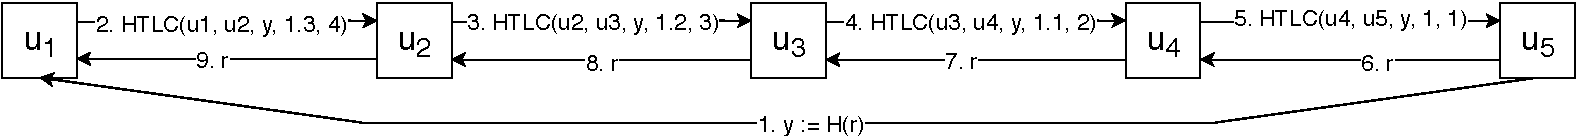
\includegraphics[width=\textwidth]{htlc-figure}
	\caption{An HTLC-based payment in the LN. The node $u_1$ pays $u_5$ using $u_2$, $u_3$ and $u_4$ as intermediaries. 
		Here we assume that each node charges a fee of $0.1$ and time is measured in days.\label{fig:htlc}}
\end{figure*}

\paragraph{Single-channel transactions}

To send a payment to Bob, Alice negotiates a new channel state.
Each channel state is reflected in a \textit{commitment transaction}.
A commitment transaction spends the output of the funding transaction and re-distributes the coins between Alice and Bob.

More precisely, each channel state is encoded in a \textit{pair} of commitment transactions: one for Alice and one for Bob.
These transactions are symmetric: they enforce a timelock on the party that holds the transaction.
In particular, Alice's version of commitment transactions allow her to redeem her output only after a timeout, and Bob's version imposes analogous restrictions on his output.
This enables the revocation mechanism (described below), which provides economic security guarantees to LN channels, assuming the parties are watching the blockchain sufficiently often.

Outputs of commitment transactions are called \textit{Hash time-locked contracts}, or \textit{HTLC}s.
HTLC is defined by a Bitcoin script that gives the funds either to one party, if it provides a pre-image of a given hash, or to the other party after a timeout.

An HTLC is an excerpt from the Bitcoin's scripting language that 
permit a node ($u_1$) to lock $x$~coins in a channel between two nodes ($u_1$ and $u_2$) 
and release them according to the encoded conditions.
The terms for the HTLC($u_1, u_2, y, x, t$) are defined with a hash value $y := H(r)$, 
where $r$ is chosen uniformly at random, 
an amount $x$ of coins, and a timeout $t$, as follows: 
(i) If $u_2$ reveals a value $r$ such that $H(r) = y$ before $t$ expires, $u_1$ pays $x$ to $u_2$; 
(ii) if $t$ expires, $u_1$ receives $x$ back.

For instance, if Alice wants to send $x$ coins to Bob, she first asks him for a \textit{payment hash}.
Bob generates a random number $r$ and send its hash $H(r)$ to Alice in a message called an \textit{invoice}.
Alice then \textit{offers} Bob an HTLC that would give him $x$~coins if he provides the preimage of $H(r)$ before time $t$, or return the coins to Alice otherwise.
Therefore an HTLC can be \textit{resolved} in one of two ways: either Bob provides the preimage and \textit{redeems} the coins before time $t$, or Alice gets the coins back.
A payment channel can keep track of multiple unresolved HTLCs concurrently, which are also called \textit{in-flight} HTLCs.


\paragraph{Multi-channel transactions}

A multi-channel transaction leverages a path of channels between a sender and a receiver (who might not share a channel between them).
%A chain of single-channel updates are set up using HTLCs with the \textit{same} hash value.
%This ensures atomicity: either all channels are re-balanced or none of them are.

LN relies on HTLCs to enable multi-hop transactions. 
The final recipient generates a random $r$ and sends its hash $H(r)$ to the initial sender.
All HTLCs along the path use the same hash value $y=H(r)$ aiming to achieve atomicity expecting that none of the intermediate balances can be updated before the receiver reveals $r$, and all of them can be updated after that.
The receiver redeems the payment from the last channel by revealing $r$, which in turn allows all intermediary channels to be re-balanced accordingly.

An illustrative example of an HTLC-based transaction is depicted in~\cref{fig:htlc}.
Here, the user $u_1$ transfers $1$~coin to $u_5$ using $u_2$, $u_3$ and $u_4$ as intermediaries.
For that, $u_5$ locally chooses a value $r$ uniformly at random, computes the cryptographic challenge for the HTLC as $y := H(r)$, and sends $y$ to the sender in an \textit{invoice} (step 1).
Then, the payment starts with a commit phase (steps 2-5) where every pair of nodes, starting from the sender, establishes an HTLC using $y$.
After the commit phase is finished, the transaction enters the release phase.
Here, the receiver reveals $r$ to $u_4$ to fulfill the contract (step 6), triggering the release phase where every pair of nodes fulfills their contract from the receiver to the sender (steps 6-9).

Intermediary users may charge a fee for the forwarding service provided. 
For instance, $u_2$ receives $1.3$~coins but only forwards $1.2$~coins, getting a fee of $0.1$~coins.
No fees are collected if a payment fails, as all pending balance updates roll back.
In the actual LN protocol, the fee consists of two parts: a constant \textit{base fee} for each payment and a \textit{fee rate} proportional to the value being transferred.
\footnote{Note that LN fee structure is different from fees on L1, where the fee is proportional to transaction weight (roughly speaking, size in bytes) but does not account for the amount of value being transferred. This may result in the economics of LN fees being significantly different from that in Bitcoin. As of 2020, LN fees are largely non-economical~\cite{Beres2019}.}

Note that the time parameter of the contracts along the path is decreasing to ensure a safety margin between HTLC timeouts.
For instance, the HTLC between $u_1$ and $u_2$ sets a timeout of four days, whereas the timeout in the HTLC between $u_2$ and $u_3$ is only three days.
This ensures that $u_2$ has enough time to settle the contract with $u_1$ after receiving $r$ from $u_3$, even if $u_3$ reveals the preimage just before the corresponding timeout expires.
There is an inherent trade-off regarding timeout lengths.
Channels with short timeouts open the risk of not being able to dispute a fraudulent transaction in case of blockchain congestion, and long timelocks open up a DoS vector, where an attacker can route many unsettled payments through a channel and effectively block it until the timelock expires.

Multi-path payments use onion routing to enforce the order of intermediary nodes.
Each intermediary node only knows the immediate previous and next nodes, but not the final sender or receiver and not its position in the path.


\subsubsection*{Channel closure}

A channel is closed when a transaction that spends the funding transaction's output gets confirmed on-chain.
This may happen in one of three ways:

\begin{itemize}
	\item Collaborative closure. Alice signals the intent to close the channel, and Bob cooperates in signing the transaction that reflects the latest channel state. This results in one on-chain transaction to close a channel, and no delays for both parties. Both parties must be online and cooperating.
	\item Non-cooperative closure without breach. Alice signals the intent to close the channel, but Bob does not respond. In this case, Alice commits the latest commitment transaction on the blockchain. Bob can redeem his output immediately, but Alice has to wait until a timeout expires. This is a safety measure to provide Bob with an opportunity to broadcast a \textit{justice transaction} (see below).
	\item Non-cooperative closure with breach. Alice broadcasts an old commitment transaction in an attempt to close the channel with an outdated distribution of funds (thus potentially stealing from Bob). If Bob does not react before the timelock on Alice's output expires, Alice can redeem her output, and the channel is closed.\footnote{From the on-chain point of view, a non disputed non-cooperative close is indistinguishable from a non-cooperative close without a breach: the blockchain does not know whether a commitment transaction is the last one, unless this fact is disputed.} If Bob is online and notices the breach before the timeout, he broadcasts the latest commitment transaction, which allows Bob to spend Alice's output before she can, punishing her for the cheating attempt.
\end{itemize}

This revocation mechanism is the key element of LN, which allows LN channels to have an unlimited lifetime (the parties do not have to close the channel if none of them wants to) and to support payments in both directions.
This makes the LN superior to earlier payment channel designs.
However, the trade-off here is that parties must be online to notice potential malicious channel closures and broadcast justice transactions.
This functionality can be outsourced.
Entities that watch the blockchains for malicious channel closures and dispute them on behalf of a user are called \textit{watchtowers}.
Implementing effective, economically incentivized, and privacy-preserving watchtowers in an active area of research~\cite{McCorry2019}.

LN's revocation mechanism has proved effective as a deterrence against malicious channel closures.
As of July~2019, there has been only 241 channel closures followed by a justice transaction -- 0.7\% of the number of Lightning channels at that time~\cite{BitMEXLN3}.
\footnote{The research is based on the LN's on-chain footprint and is not absolutely accurate. A non-cooperative closure followed by a justice transaction may also happen without malicious intent, for example, as a result of a broken backup restore (where Alice's node "forgets" about the latest state and broadcasts an earlier state assuming it is the latest one).}


\subsection{P2P network and routing}

In the description of multi-channel transactions, we noted that the sender arranges a series of HTLCs along the path towards the receiver.
But how does the sender construct such a path?

LN nodes gossip about newly opened channels that are marked as available for routing.
Based on this information, each node maintains a local view of the network, and uses it to calculate routes to the receiver.
As total channel capacities are known, the sender only considers channels with the capacity larger than $X$ for a payment of amount $X$.
However, this is insufficient to prevent routing failures, because the distribution of funds in channels is not known.
The ability of channel parties to send or forward payments is limited by their \textit{local} channel balances.
Initially, if Alice opens a channel with Bob, all funds are on her side.
This means that she can send up to the total capacity, but she can not receive.
As the local balances change, the routing capabilities of the channels in both directions are also changing.
This makes routing not very reliable, especially for larger payment amounts.

In case of payment failure, an error message notifies the sender which channel has failed.
The sender would presumably try to send the payment again along a new route without the failed channel.
This procedure repeats multiple times until a payment succeeds.
Optimizing path finding for payment channel networks is an active area of research~\cite{Pickhardt2019a, Prihodko2016, Grunspan2018, Pickhardt2019, Piatkivskyi2018, Sivaraman2018, Bagaria2019, Roos2018}.


\section{Privacy in payment channel networks}

There are substantial differences in the privacy models of first- and second-layer blockchain protocols.
In contrast to Bitcoin transactions, which are openly broadcast, LN payments are only sent to a short chain of randomly chosen nodes.
Due to onion routing, each intermediary node only knows the previous and the next hops, but not the whole route and even not its position in the route.
This leads to an assumption that Lightning provides more privacy than Bitcoin.

\todo[inline]{Outline differences}



